3. \begin{figure}[ht!]
\center{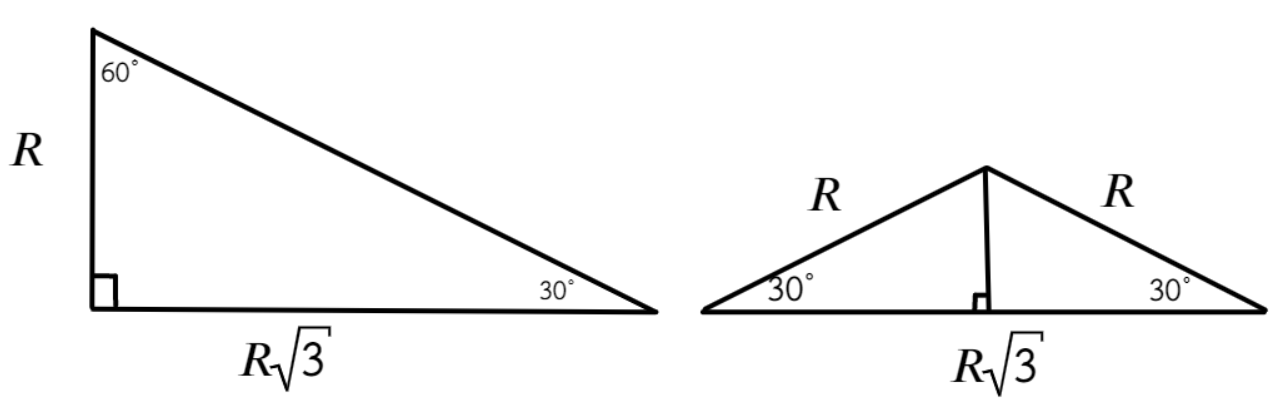
\includegraphics[scale=0.35]{g9-3.png}}
\end{figure}\\
Пусть напротив сторон с величинами $R$ и $R\sqrt{3}$ лежат углы $\alpha$ и $\beta.$ Тогда по теореме синусов $\cfrac{R}{\sin(\alpha)}=\cfrac{R\sqrt{3}}{\sin(\beta)}=2R\Rightarrow \alpha=30^\circ\text{ или }150^\circ,\ \beta=60^\circ\text{ или }120^\circ.$
Возможны два случая $\alpha=30^\circ,\ \beta=60^\circ$ или $\alpha=30^\circ,\ \beta=120^\circ.$ Если $\alpha=150^\circ,$ то сумма углов треугольника получается больше $180^\circ$ при любом возможном значении $\beta.$ В первом случае треугольник является прямоугольным и его площадь равна $S=\cfrac{R\cdot R\sqrt{3}}{2}=\cfrac{\sqrt{3}}{2}R^2.$ Во втором случае треугольник является равнобедренным ($180^\circ-120^\circ-30^\circ=30^\circ$), опустим высоту из его вершины, она равна $R\sin(30^\circ)=\cfrac{1}{2}R.$ Тогда площадь треугольника равна $S=\cfrac{1}{2}\cdot\cfrac{1}{2}R\cdot R\sqrt{3}=\cfrac{\sqrt{3}}{4}R^2.$
ewpage
oindent
